\documentclass[german,oneside,color]{htldipl}
% Zulässige Class Options: 
%   Hauptsprache: german (default), english
%   Doppelseitig: oneside (default), twoside
%   Syntax-Highlighting: color (default), black

% die folgende Zeile einkommentieren für Arial-Ähnliche Schriftart
%\renewcommand{\familydefault}{\sfdefault}

\graphicspath{{images/}}    % wo liegen die Bilder?
\usepackage[paper=a4paper,margin=3cm]{geometry}

\makeindex[title=Index]
\makeindex[name=allgemein, title=Allgemeiner Index]
\makeindex[name=name,title={Autoren Index}]
\makeindex[name=title,columns=1,title={Literatur Index}]
\indexsetup{level=\subsection*, toclevel=subsection, noclearpage}


\makeatletter
\@ifpackageloaded{biblatex_legacy}
  {\DeclareIndexNameFormat{default}{%
     \usebibmacro{index:name}{\index[name]}{#1}{#3}{#5}{#7}}}
  {\DeclareIndexNameFormat{default}{%
     \usebibmacro{index:name}{\index[name]}
       {\namepartfamily}
       {\namepartgiven}
       {\namepartprefix}
       {\namepartsuffix}}}
\makeatother

\DeclareIndexFieldFormat{indextitle}{%
  \usebibmacro{index:title}{\index[title]}{#1}}

\renewbibmacro*{bibindex}{%
  \ifbibindex
    {\indexnames{author}%
     \indexnames{editor}%
     \indexnames{translator}%
     \indexnames{commentator}%
     \indexfield{indextitle}}
    {}}

\makeglossaries
%\include{glossary}
\loadglsentries{glossary}
\addbibresource{literatur.bib}     %BibTeX-Datei literatur.bib

%%%----------------------------------------------------------
\begin{document}
%%%----------------------------------------------------------

\title{Entwurf eines Versuchstandes für Kreiselpumpen}
\abteilung{Maschineningenieurwesen}
%\schwerpunkt{} wenn kein Ausbildungsschwerpunkt vorhanden ist z.B. Informatik
\schwerpunkt{Ausbildungsschwerpunkt Automatisierungstechnik}
\studienort{Wiener Neustadt}
\schule{HTBLuVA Wiener Neustadt}
\schullogo{htl.jpeg}
\abgabejahr{2010/11}
\betreuerA{Dr.\ Walter Turbo}
\betreuerB{Dipl.-Ing.\ Hans Kreisel}
\betreuerC{Kurt Heidenheim}
\betreuerD{Ing.\ Reiner Tischler}
%\betreuerD{} leer lassen wenn nicht vorhanden
\schuelerA{Maximilian MAIER}
\evidenzA{5AHMIA-17}
\subthemaA{Konstruktion des Versuchstandes}
\schuelerB{Elisabeth MUSTER}
\evidenzB{5AHMIA-19}
\subthemaB{Erstellen der Pumpenkennlinien}
\schuelerC{Peter ZAPFEL}
\evidenzC{5AHMIA-24}
\subthemaC{Integration des Versuchstandes in die bestehende Softwarelösung für die Kennlinien}
\schuelerD{Otto BAUER}
\evidenzD{5BHMIA-02}
\subthemaD{Subthema D}
\schuelerE{Elfriede NURNBERG-ATTACH}
\evidenzE{5BHMIA-20}
\subthemaE{Subthema E}
%\schuelerE{} leer lassen wenn nicht vorhanden
%\evidenzE{}
%\subthemaE{}

%%%----------------------------------------------------------
\frontmatter
\maketitle
\tableofcontents
%%%----------------------------------------------------------

\include{vorwort}				%ggfs. weglassen
\includepdf[pages=1-1,pagecommand={\chapter[Diplomarbeit Dokumentation]{}}]{pdf/Formular-printed.pdf}
\includepdf[pages=2-2,pagecommand={\thispagestyle{plain}}]{pdf/Formular-printed.pdf}
\includepdf[pages=3-3,pagecommand={\chapter[Diploma Thesis Documentation]{}}]{pdf/Formular-printed.pdf}
\includepdf[pages=4-4,pagecommand={\thispagestyle{plain}}]{pdf/Formular-printed.pdf}
\include{kurzfassung}		
\include{abstract}			

%%%----------------------------------------------------------
\mainmatter           %Hauptteil (ab hier arab. Seitenzahlen)
%%%----------------------------------------------------------

\include{einleitung}
\include{diplomschrift}
\include{latex}
\chapter{Häufige Fragen und Probleme mit Latex}

Im Laufe der Arbeit mit Latex stoßen Schüler immer wieder auf sehr ähnliche Probleme und Fehler. 
Dieses Kapitel stellt eine Sammlung der häufigsten Probleme und Fehler dar und soll als erste Anlaufstelle zur Problemlösung dienen.

\subsubsection*{Umlaute (ö, Ö, ü, Ü, ä, A, ß, ...) werden im erzeugten PDF nicht korrekt dargestellt oder erzeugen Fehler beim Erzeugen des PDFs.}
Dieser Fehler wird fast immer durch eine falsche Zeichenkodierung\footnote{\url{https://de.wikipedia.org/wiki/Zeichenkodierung}} der Textdatei erzeugt. 
Die Vorlage erwartet durchgehend mit UTF-8\footnote{\url{https://de.wikipedia.org/wiki/UTF-8}} erzeugte Textdateien. 
Leider erzeugen einige Editoren bzw. Betriebssysteme standardmäßig keine UTF-8 Textdateien. Abhilfe schafft ein einfaches neu speichern der Textdatei als UTF-8. 
Die Zeichenkodierung kann bei den meisten Editoren im Speichern unter Dialog ausgewählt werden.
%Abbildung Speichern unter Dialog

\subsubsection*{Beim Erzeugen des PDFs kommt eine Fehlermeldung das Paket XYZ.sty fehlt.}
Dieser Fehler hängt von der verwendeten Latex-Installation ab. Bei Miktex können fehlende Pakete automatisch nachinstalliert werden. 
Manchmal funktioniert diese Automatik jedoch nicht. In diesem Fall ist es am Einfachsten die fehlende Pakete im Miktex-Manager manuell zu installieren. 
Bei Linux und anderen Betriebssystemen kann die Latex-Umgebung meist als Full-Install installiert werden. Hier werden alle verfügbaren Pakete installiert. 
Alternativ kann man mit Google ermitteln welches Installationspaket\footnote{Übersicht der Latex-Pakete für Mac \url{https://trac.macports.org/wiki/TeXLivePackages}} die benötigen XYZ.sty Dateien zur Verfügung stellt.
\include{abbildungen}
\include{mathematik}
\include{literatur}
\include{drucken}
\include{word}
\include{schluss}

%%%----------------------------------------------------------
%%%Anhang
\appendix
%\include{anhang_a}	% Technische Ergänzungen
\include{anhang_b}	% Inhalt der CD-ROM/DVD
\include{anhang_c}	% Chronologische Liste der Änderungen
\include{anhang_d}	% Quelltext dieses Dokuments

%%%----------------------------------------------------------

\clearpage
\printglossaries

\clearpage
\chapter*{Index}
\addcontentsline{toc}{chapter}{Index}
\printindex[allgemein]

\printindex

\printindex[name]

\printindex[title]


%Literaturverzeichnis
\clearpage
\addcontentsline{toc}{chapter}{\bibname}

\printbibliography


%%%----------------------------------------------------------

%%%Messbox zur Druckkontrolle
\include{messbox}

\end{document}
